% !TeX spellcheck = cs_CZ
%{\tikzset{external/prefix={tikz/FYZII/}}
% \tikzset{external/figure name/.add={ch29_}{}}
%---------------------------------------------------------------------------------------------------
% file fey2ch29.tex
%---------------------------------------------------------------------------------------------------
%=========================== Kapitola Pohyb nábojů v elektrickém a magnetickém poli ================
\setchaptertoc
\chapter{Pohyb nábojů v elektrickém a magnetickém poli}\label{fyz:IIchapXXIX}

  \section{Pohyb v homogenní elektrickém nebo magnetickém poli}\label{fyz:IIchapXXIXsecI}
  \section{Analyzátor hybnosti}\label{fyz:IIchapXXIXsecII}
  \section{Elektrostatická čočka}\label{fyz:IIchapXXIXsecIII}
  \section{Magnetická čočka}\label{fyz:IIchapXXIXsecIV}
  \section{Elektronový mikroskop}\label{fyz:IIchapXXIXsecV}
  \section{Stabilizující pole urychlovačů}\label{fyz:IIchapXXIXsecVI}
  \section{Fokusace pomocí střídavého gradientu}\label{fyz:IIchapXXIXsecVII}
  \section{Pohyb ve skřížených elektrických a magnetických polích}\label{fyz:IIchapXXIXsecVIII}
  \section{Příklady a cvičení}\label{fyz:IIchapXXIXsecIX}


    \begin{figure}[ht!] %\ref{fyz:fig0623}
      \centering
      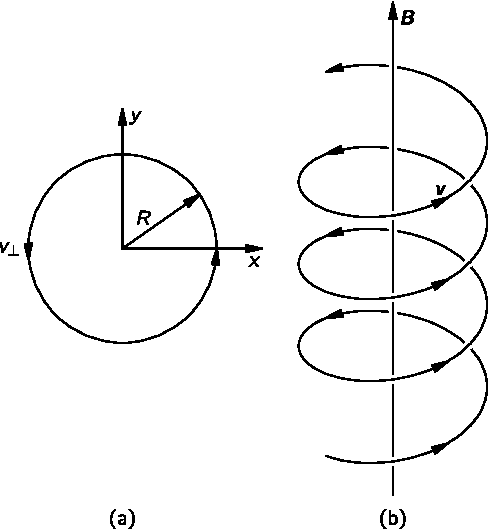
\includegraphics[width=0.7\linewidth]{fyz_fig0623.pdf}
      \caption{
               (\cite[s.~707]{Feynman02})}
      \label{fyz:fig0623}
    \end{figure}

    \begin{figure}[ht!]
      \centering
      \subcaptionbox{\label{fyz:fig0624a}}{\luafigure[0.45]{fyz_fig0624a.pdf}}
      \subcaptionbox{\label{fyz:fig0624b}}{\luafigure[0.45]{fyz_fig0624b.pdf}}
      \label{fyz:fig0624}
      \caption{
               (\cite[s.~748]{Feynman02})}
    \end{figure}

    \begin{figure}[ht!] %\ref{fyz:fig0625}
      \centering
      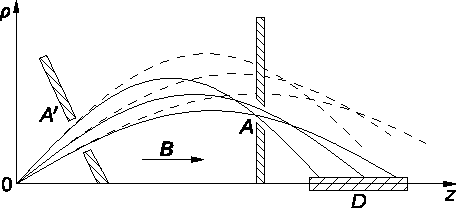
\includegraphics[width=0.7\linewidth]{fyz_fig0625.pdf}
      \caption{
               (\cite[s.~707]{Feynman02})}
      \label{fyz:fig0625}
    \end{figure}

    \begin{figure}[ht!] %\ref{fyz:fig0626}
      \centering
      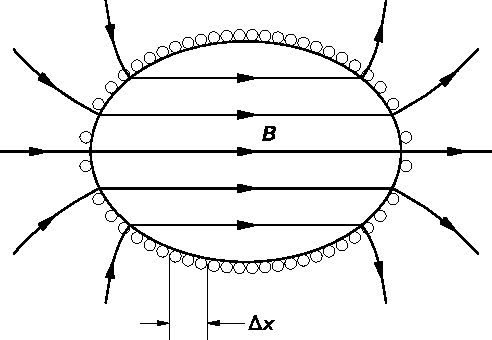
\includegraphics[width=0.7\linewidth]{fyz_fig0626.pdf}
      \caption{
               (\cite[s.~707]{Feynman02})}
      \label{fyz:fig0626}
    \end{figure}

    \begin{figure}[ht!] %\ref{fyz:fig0627}
      \centering
      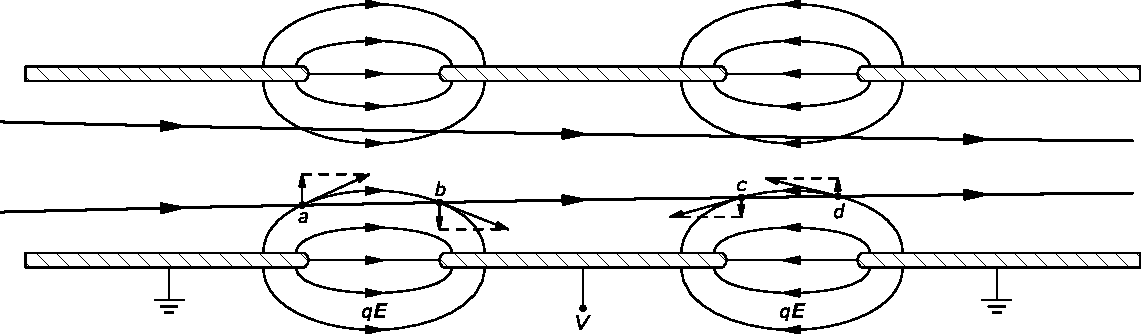
\includegraphics[width=0.7\linewidth]{fyz_fig0627.pdf}
      \caption{
               (\cite[s.~707]{Feynman02})}
      \label{fyz:fig0627}
    \end{figure}

    \begin{figure}[ht!] %\ref{fyz:fig0628}
      \centering
      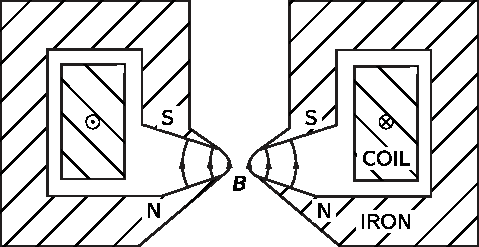
\includegraphics[width=0.7\linewidth]{fyz_fig0628.pdf}
      \caption{
               (\cite[s.~707]{Feynman02})}
      \label{fyz:fig0628}
    \end{figure}

    \begin{figure}[ht!] %\ref{fyz:fig0629}
      \centering
      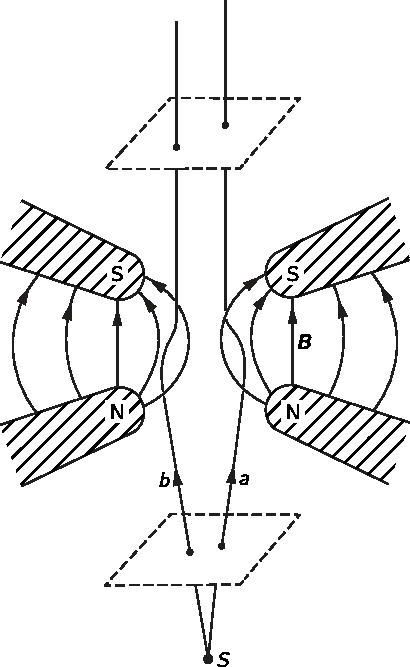
\includegraphics[width=0.7\linewidth]{fyz_fig0629.pdf}
      \caption{
               (\cite[s.~707]{Feynman02})}
      \label{fyz:fig0629}
    \end{figure}

    \begin{figure}[ht!] %\ref{fyz:fig0630}
      \centering
      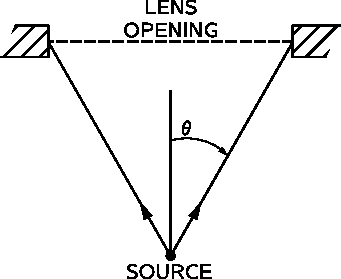
\includegraphics[width=0.7\linewidth]{fyz_fig0630.pdf}
      \caption{
               (\cite[s.~707]{Feynman02})}
      \label{fyz:fig0630}
    \end{figure}

    \begin{figure}[ht!] %\ref{fyz:fig0631}
      \centering
      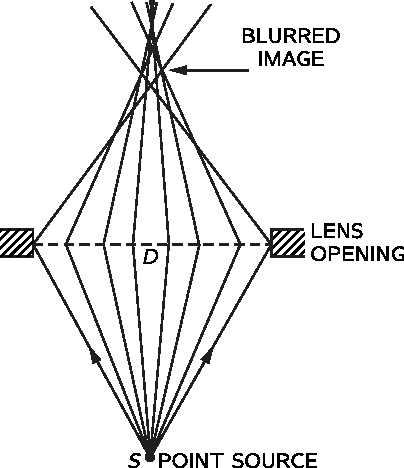
\includegraphics[width=0.7\linewidth]{fyz_fig0631.pdf}
      \caption{
               (\cite[s.~707]{Feynman02})}
      \label{fyz:fig0631}
    \end{figure}

    \begin{figure}[ht!] %\ref{fyz:fig0632}
      \centering
      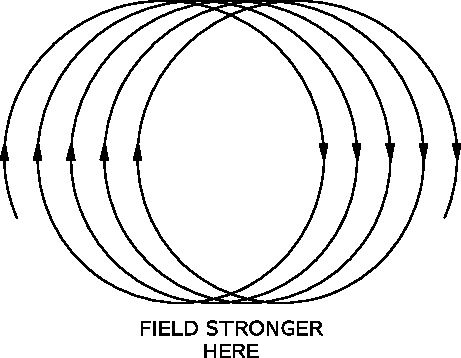
\includegraphics[width=0.7\linewidth]{fyz_fig0632.pdf}
      \caption{
               (\cite[s.~707]{Feynman02})}
      \label{fyz:fig0632}
    \end{figure}

    \begin{figure}[ht!] %\ref{fyz:fig0633}
      \centering
      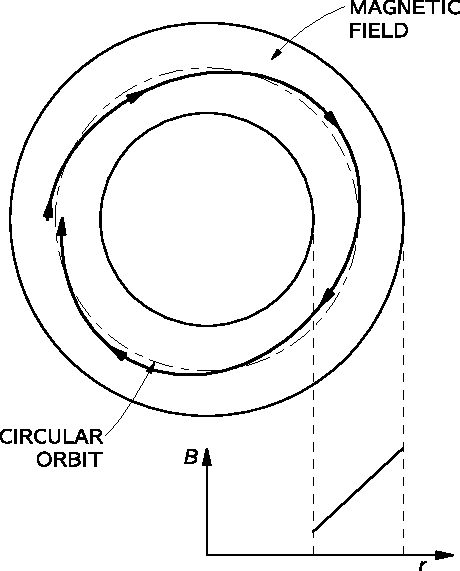
\includegraphics[width=0.7\linewidth]{fyz_fig0633.pdf}
      \caption{
               (\cite[s.~707]{Feynman02})}
      \label{fyz:fig0633}
    \end{figure}

    \begin{figure}[ht!] %\ref{fyz:fig0634}
      \centering
      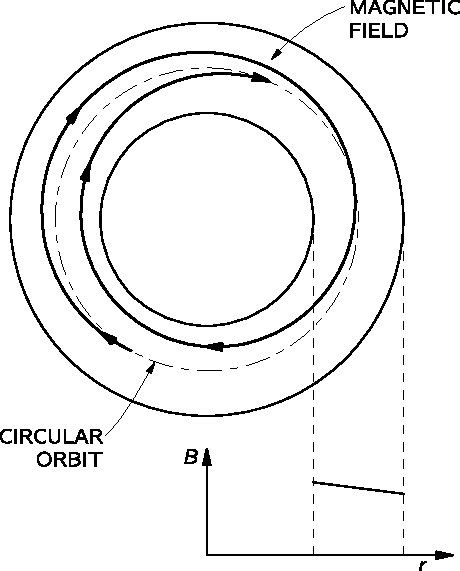
\includegraphics[width=0.7\linewidth]{fyz_fig0634.pdf}
      \caption{
               (\cite[s.~707]{Feynman02})}
      \label{fyz:fig0634}
    \end{figure}

    \begin{figure}[ht!] %\ref{fyz:fig0635}
      \centering
      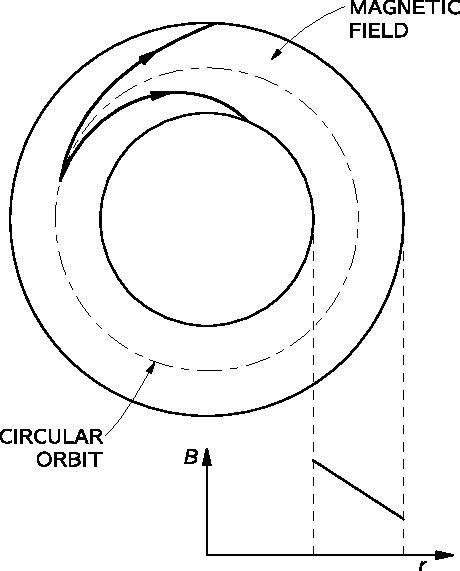
\includegraphics[width=0.7\linewidth]{fyz_fig0635.pdf}
      \caption{
               (\cite[s.~707]{Feynman02})}
      \label{fyz:fig0635}
    \end{figure}

    \begin{figure}[ht!] %\ref{fyz:fig0636}
      \centering
      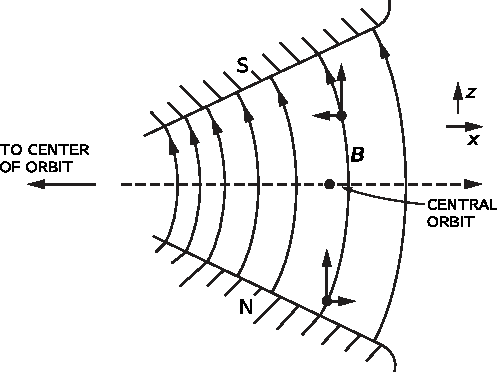
\includegraphics[width=0.7\linewidth]{fyz_fig0636.pdf}
      \caption{
               (\cite[s.~707]{Feynman02})}
      \label{fyz:fig0636}
    \end{figure}

    \begin{figure}[ht!] %\ref{fyz:fig0637}
      \centering
      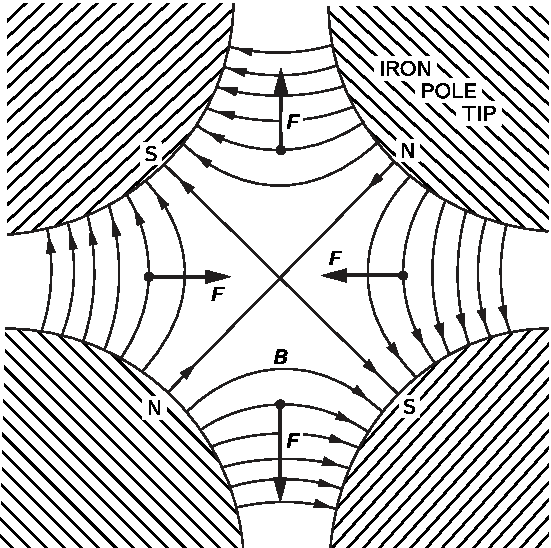
\includegraphics[width=0.7\linewidth]{fyz_fig0637.pdf}
      \caption{
               (\cite[s.~707]{Feynman02})}
      \label{fyz:fig0637}
    \end{figure}

    \begin{figure}[ht!] %\ref{fyz:fig0638}
      \centering
      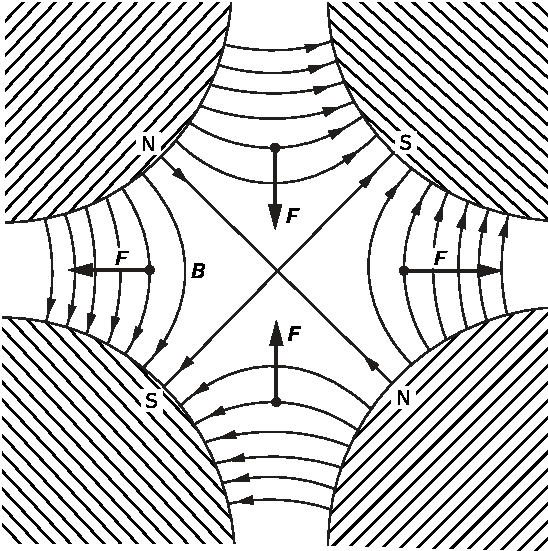
\includegraphics[width=0.7\linewidth]{fyz_fig0638.pdf}
      \caption{
               (\cite[s.~707]{Feynman02})}
      \label{fyz:fig0638}
    \end{figure}

    \begin{figure}[ht!] %\ref{fyz:fig0639}
      \centering
      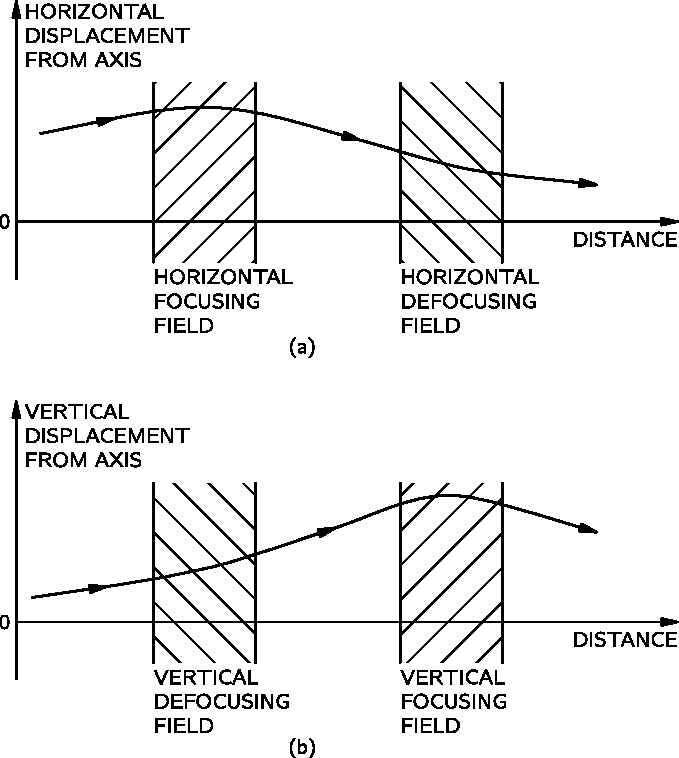
\includegraphics[width=0.7\linewidth]{fyz_fig0639.pdf}
      \caption{
               (\cite[s.~707]{Feynman02})}
      \label{fyz:fig0639}
    \end{figure}

    \begin{figure}[ht!] %\ref{fyz:fig0640}
      \centering
      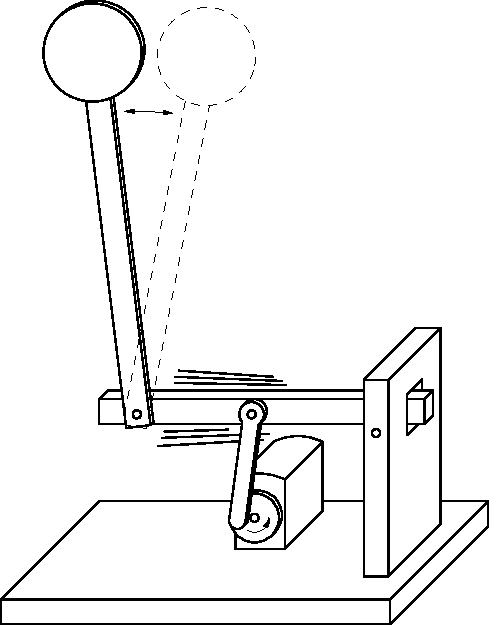
\includegraphics[width=0.7\linewidth]{fyz_fig0640.pdf}
      \caption{
               (\cite[s.~707]{Feynman02})}
      \label{fyz:fig0640}
    \end{figure}

    \begin{figure}[ht!] %\ref{fyz:fig0641}
      \centering
      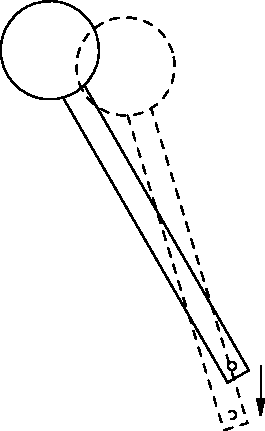
\includegraphics[width=0.7\linewidth]{fyz_fig0641.pdf}
      \caption{
               (\cite[s.~707]{Feynman02})}
      \label{fyz:fig0641}
    \end{figure}

    \begin{figure}[ht!] %\ref{fyz:fig0642}
      \centering
      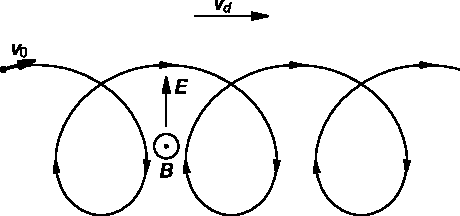
\includegraphics[width=0.7\linewidth]{fyz_fig0642.pdf}
      \caption{
               (\cite[s.~707]{Feynman02})}
      \label{fyz:fig0642}
    \end{figure}

    \todo[inline]{Kapitola fey2ch29 je nedodělaná, obsahuje pouze obrázky}
%} %tikzset
%---------------------------------------------------------------------------------------------------